\documentclass{beamer}
\usepackage[utf8]{inputenc}

\usetheme{Madrid}
\usecolortheme{default}
\usepackage{amsmath,amssymb,amsfonts,amsthm}
\usepackage{txfonts}
\usepackage{tkz-euclide}
\usepackage{listings}
\usepackage{adjustbox}
\usepackage{array}
\usepackage{tabularx}
\usepackage{gvv}
\usepackage{lmodern}
\usepackage{circuitikz}
\usepackage{tikz}
\usepackage{graphicx}
\usepackage{multicol}
\setbeamertemplate{page number in head/foot}[totalframenumber]

\usepackage{tcolorbox}
\tcbuselibrary{minted,breakable,xparse,skins}



\definecolor{bg}{gray}{0.95}
\DeclareTCBListing{mintedbox}{O{}m!O{}}{%
  breakable=true,
  listing engine=minted,
  listing only,
  minted language=#2,
  minted style=default,
  minted options={%
    linenos,
    gobble=0,
    breaklines=true,
    breakafter=,,
    fontsize=\small,
    numbersep=8pt,
    #1},
  boxsep=0pt,
  left skip=0pt,
  right skip=0pt,
  left=25pt,
  right=0pt,
  top=3pt,
  bottom=3pt,
  arc=5pt,
  leftrule=0pt,
  rightrule=0pt,
  bottomrule=2pt,

  colback=bg,
  colframe=orange!70,
  enhanced,
  overlay={%
    \begin{tcbclipinterior}
    \fill[orange!20!white] (frame.south west) rectangle ([xshift=20pt]frame.north west);
    \end{tcbclipinterior}},
  #3,
}
\lstset{
    language=C,
    basicstyle=\ttfamily\small,
    keywordstyle=\color{blue},
    stringstyle=\color{orange},
    commentstyle=\color{green!60!black},
    numbers=left,
    numberstyle=\tiny\color{gray},
    breaklines=true,
    showstringspaces=false,
}
%------------------------------------------------------------
%This block of code defines the information to appear in the
%Title page
\title %optional
{1.1.12}
\date{October  2025}
%\subtitle{A short story}

\author % (optional)
{BEERAM MADHURI - EE25BTECH11012}



\begin{document}


\frame{\titlepage}
\begin{frame}{Question}
Given closed-loop transfer function $T(s) = \frac{s-5}{(s+2)(s+3)}$, the system is: \hfill (EC 2007)

\begin{enumerate}
    \item[a)] Unstable
    \item[b)] Uncontrollable
    \item[c)] Minimum phase
    \item[d)] Non-minimum phase
\end{enumerate}
\end{frame}

\begin{frame}{solution}
    \frametitle{finding the Property of given system}
Given the closed-loop transfer function:
\begin{align}
    T(s) = \frac{s - 5}{(s + 2)(s + 3)}
\end{align}
Identifiying Poles and Zeros\\
\textbf{Poles:}\\
Set the denominator to zero: \\
\begin{align}
    (s + 2)(s + 3) = 0\\
    s = -2 ,-3
\end{align}
 Both are in the Left Half Plane (LHP).
\end{frame}
\begin{frame}
    \textbf{Zeros:}\\
Set the numerator to zero: 
\begin{align}{}
    s - 5 = 0\\
    s = +5
\end{align}
This is in the Right Half Plane (RHP).
\end{frame}
\begin{frame}{}
    Given Options:\\
a) Unstable:\\
A system is unstable if any of its poles lie in the Right Half Plane (RHP) or if there are repeated poles on the imaginary axis. (Our system is stable because poles are at -2 and -3).\\
b)Uncontrollable:\\
A property related to State-Space analysis. In transfer functions, it usually implies a pole-zero cancellation. Since no terms cancel out here, we cannot assume it is uncontrollable from this form.
\end{frame}
\begin{frame}
c)Minimum Phase:\\
A system where all poles and all zeros lie in the Left Half Plane (LHP). These systems have the minimum possible phase shift for a given magnitude response.\\
d)Non-minimum Phase:\\
A system that has at least one zero (or pole) in the Right Half Plane (RHP). These systems exhibit "undershoot" in their step response and have more phase lag than a minimum phase system.\\
\end{frame}
\begin{frame}
Determining the System Property:
Since we have a zero at $s = 5$, the system is non-minimum phase.\\
Correct Option: d) Non-minimum phase
\end{frame}

\begin{frame}[fragile]
    \frametitle{Python Code}
    \begin{lstlisting}
import matplotlib
matplotlib.use('Agg')  # Required for Termux/Debian
import matplotlib.pyplot as plt
import control as ctrl
import numpy as np
# Define T(s) = (s - 5) / (s^2 + 5s + 6)
num = [1, -5]
den = [1, 5, 6]
sys = ctrl.TransferFunction(num, den)
\end{lstlisting}
\end{frame}

\begin{frame}[fragile]
\frametitle{Python Code}
\begin{lstlisting}
# Extract poles and zeros for manual labeling
poles = ctrl.poles(sys)
zeros = ctrl.zeros(sys)

plt.figure(figsize=(10, 7))
\end{lstlisting}
\end{frame}

\begin{frame}[fragile]
\frametitle{Python Code}
\begin{lstlisting}
# Generate the PZ map using the control library
# This handles the 'x' and 'o' markers automatically
ctrl.pole_zero_plot(sys, plot=True, title='Pole-Zero Map with Labels')

# Plot Poles (Red X)
for p in poles:
    plt.plot(p.real, p.imag, 'rx', markersize=10, mew=2)
    plt.text(p.real, p.imag + 0.1, f' Pole: {p.real:.1f}', 
             color='red', fontweight='bold', ha='center')
\end{lstlisting}
\end{frame}

\begin{frame}[fragile]
\frametitle{Python Code}
\begin{lstlisting}
# Plot Zeros (Blue o)
for z in zeros:
    plt.plot(z.real, z.imag, 'bo', markersize=10, fillstyle='none', mew=2)
    plt.text(z.real, z.imag + 0.1, f' Zero: {z.real:.1f}', 
             color='blue', fontweight='bold', ha='center')
plt.axvspan(0, max(zeros.real) + 2, color='yellow', alpha=0.1)
if any(z.real > 0 for z in zeros):
    plt.text(2.5, -0.5, "NON-MINIMUM PHASE\n(Zero in RHP)", 
             bbox=dict(facecolor='white', alpha=0.8), ha='center', color='darkred')
\end{lstlisting}
\end{frame}

\begin{frame}[fragile]
\frametitle{Python Code}
\begin{lstlisting}
# Final Touches
plt.grid(True, which='both', linestyle='--', alpha=0.5)
plt.axvline(0, color='black', linewidth=1.5)
plt.axhline(0, color='black', linewidth=1.5)
plt.xlabel('Real Axis')
plt.ylabel('Imaginary Axis')

# Save and Notify
plt.savefig('labeled_system_plot.png')
print("Successfully generated 'labeled_system_plot.png'")
\end{lstlisting}
\end{frame}

\begin{frame}[fragile]
\frametitle{C Code}
\begin{lstlisting}
#include <stdio.h>
#include <math.h>

typedef struct {
    double real;
    double imag;
} Complex;

int main() {
    // Numerator: s - 5 = 0
    // Zero: s = 5
    double zero = 5.0;
\end{lstlisting}
\end{frame}

\begin{frame}[fragile]
\frametitle{C Code}
\begin{lstlisting}
    // Denominator: (s + 2)(s + 3) = s^2 + 5s + 6 = 0
    // Using Quadratic Formula: s = [-b +/- sqrt(b^2 - 4ac)] / 2a
    double a = 1.0, b = 5.0, c = 6.0;
    double discriminant = b*b - 4*a*c;
    
    double pole1 = (-b + sqrt(discriminant)) / (2*a);
    double pole2 = (-b - sqrt(discriminant)) / (2*a);
\end{lstlisting}
\end{frame}

\begin{frame}[fragile]
\frametitle{C Code}
\begin{lstlisting}
    printf("--- System Analysis ---\n");
    printf("Zero: s = %.1f\n", zero);
    printf("Pole 1: s = %.1f\n", pole1);
    printf("Pole 2: s = %.1f\n", pole2);
    printf("-----------------------\n");

    // Logic to determine system properties
    if (pole1 > 0 || pole2 > 0) {
        printf("Result: System is UNSTABLE (Poles in RHP).\n");
    } else {
        printf("Result: System is STABLE (Poles in LHP).\n");
    }
\end{lstlisting}
\end{frame}

\begin{frame}[fragile]
\frametitle{C Code}
\begin{lstlisting}
    if (zero > 0) {
        printf("Result: System is NON-MINIMUM PHASE (Zero in RHP).\n");
    } else {
        printf("Result: System is MINIMUM PHASE.\n");
    }

    return 0;
}
\end{lstlisting}
\end{frame}
\begin{frame}{Plot}
\begin{figure}[H]
\centering
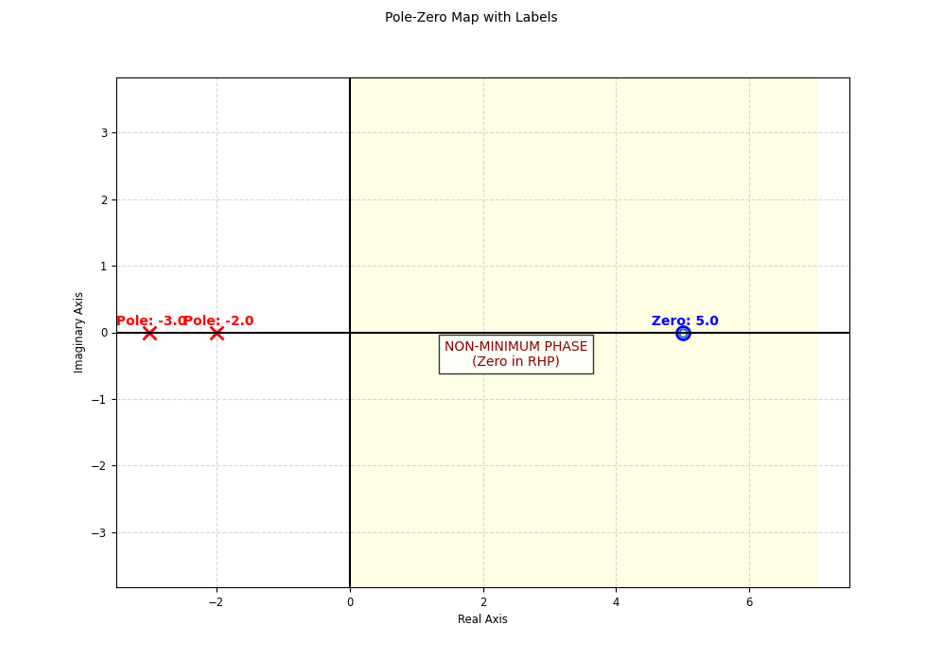
\includegraphics[width=0.75\columnwidth]{figures/plot.png}
\caption{Poles and Zeroes}
\label{fig:placeholder}
\end{figure}
\end{frame}

\end{document}